\documentclass[12pt,a4paper]{article}
\usepackage[utf8]{inputenc}
\usepackage[T1]{fontenc}
\usepackage[ngerman]{babel}
\usepackage{amsmath,amssymb,amsthm}
\usepackage{graphicx}
\usepackage{geometry}
\usepackage{booktabs}
\usepackage{hyperref}
\usepackage{xcolor}
\usepackage{float}
\usepackage{caption}
\usepackage{subcaption}
\usepackage{enumitem}
\usepackage{cite}
\usepackage{array}
\usepackage{lmodern}
\usepackage{microtype}
\usepackage{titlesec}
\usepackage{fancyhdr}
\usepackage{tocloft}
\usepackage{setspace}

\geometry{
  top=2.5cm, bottom=2.5cm,
  left=3.0cm, right=2.5cm
}

\hypersetup{
  colorlinks=true,
  linkcolor=blue!70!black,
  citecolor=green!60!black,
  urlcolor=blue!70!black,
  pdftitle={Strahltriebwerke: Typen, Thermodynamik und optimale Hybridkonzepte},
  pdfauthor={S. Epp, Universit\"at Bielefeld}
}

\setlength{\parindent}{0pt}
\setlength{\parskip}{6pt}

\newtheorem{theorem}{Theorem}[section]
\newtheorem{lemma}[theorem]{Lemma}
\newtheorem{korollar}[theorem]{Korollar}
\newtheorem{definition}[theorem]{Definition}
\theoremstyle{remark}
\newtheorem{bemerkung}[theorem]{Bemerkung}

% Convenience notation
\newcommand{\Ma}{\mathrm{Ma}}
\newcommand{\BPR}{\mathrm{BPR}}
\newcommand{\piK}{\pi_{\mathrm{K}}}
\newcommand{\etath}{\eta_{\mathrm{th}}}
\newcommand{\etaprop}{\eta_{\mathrm{prop}}}
\newcommand{\etages}{\eta_{\mathrm{ges}}}
\newcommand{\Fs}{F_{\mathrm{s}}}
\newcommand{\TSFC}{\mathrm{TSFC}}

\title{\textbf{Strahltriebwerke: Typen, Thermodynamik und optimale Hybridkonzepte}}
\author{Stephan Epp}
\date{12. April 2026}

\begin{document}

\maketitle
\tableofcontents
\newpage

% ─── 1. Einleitung ────────────────────────────────────────────────────────────
\section{Einleitung}
    Diese Arbeit untersucht systematisch die acht wichtigsten Klassen von Strahltriebwerken --
Turboshaft, Turboprop, Turbofan, Turbojet, Ramjet, Scramjet, Raketentriebwerk und Pulsejet --
hinsichtlich ihrer thermodynamischen Grundprinzipien, ihres spezifischen Schubs,
ihres Kraftstoffverbrauchs (TSFC) und ihrer Emissionen.
Auf Basis des verallgemeinerten Brayton-Kreisprozesses werden formale Definitionen,
Lemmata und Theoreme zum Wirkungsgrad formuliert und bewiesen.
Anschlie{\ss}end wird ein optimaler Hybridmotor-Typ theoretisch abgeleitet,
der durch adaptive Moduswechsel zwischen Turbofan-, Ramjet- und Scramjet-Regime
\"uber den gesamten Machzahlbereich von $\Ma = 0$ bis $\Ma = 12$
einen thermodynamischen Gesamtwirkungsgrad von bis zu $\etath = 0{,}65$
bei einem um ca. $36\,\%$ reduzierten Kraftstoffverbrauch gegen\"uber dem
Stand der Technik erreicht.
Zehn Matplotlib-Abbildungen veranschaulichen die quantitativen Zusammenh\"ange.
Im abschlie{\ss}enden Ausblick werden Forschungsrichtungen der n\"achsten Dekaden skizziert,
darunter wasserstoffbetriebene Hybridtriebwerke,
KI-gest\"utzte Ventilatorregelung und detonationsbasierte Verbrennungskonzepte.

Strahltriebwerke z\"ahlen zu den faszinierendsten technischen Errungenschaften des 20. Jahr\-hun\-derts
und bilden die tragende S\"aule der modernen Luft- und Raumfahrt.
Sie arbeiten nach dem Prinzip der Impuls\"ubertragung: Ein Fluid -- in der Regel Luft
zusammen mit verbrannten Treibstoffgasen -- wird beschleunigt und nach hinten
ausgestossen; nach dem dritten Newtonschen Gesetz entsteht ein gleichgro{\ss}er
Schub nach vorn.

Trotz dieses gemeinsamen Grundprinzips unterscheiden sich die einzelnen Triebwerksklassen
erheblich in ihrer konstruktiven Auslegung, dem Grad der internen Kompression,
dem Bypasverh\"altnis sowie in ihrem optimalen Betriebsbereich.
Turbofantriebwerke dominieren heute die kommerzielle Luftfahrt im Unterschallbereich,
w\"ahrend Scramjets auf hypersonische Fl\"uge ausgelegt sind.

\medskip
\textbf{Ziel dieser Arbeit} ist eine vollst\"andige thermodynamische Analyse aller Typen
sowie die formale Ableitung eines optimalen Hybridkonzepts, das minimalen Verbrauch
bei maximalem Wirkungsgrad \"uber den gesamten Machzahlbereich vereint.

\medskip
\textbf{Aufbau der Arbeit.}
Abschnitt~\ref{sec:grundlagen} legt die thermodynamischen Grundlagen des
Brayton-Kreisprozesses fest.
Abschnitt~\ref{sec:typen} analysiert die acht Triebwerksklassen ausf\"uhrlich.
Abschnitt~\ref{sec:vergleich} pr\"asentiert den quantitativen Vergleich.
Abschnitt~\ref{sec:hybrid} leitet das optimale Hybridtriebwerk her und beweist
die Wirkungsgradverbesserung formal.
Abschnitt~\ref{sec:emissionen} diskutiert die Emissionsbilanz.
Der abschlie{\ss}ende Ausblick in Abschnitt~\ref{sec:ausblick} skizziert
zuk\"unftige Forschungsrichtungen in unbeispielloser Tiefe.

% ─── 2. Thermodynamische Grundlagen ──────────────────────────────────────────
\section{Thermodynamische Grundlagen}
\label{sec:grundlagen}

\subsection{Der Brayton-Kreisprozess}

Das ideale Referenzmodell f\"ur Gasturbinen und Strahltriebwerke ist der
\emph{Brayton-Kreisprozess} (auch Joule-Kreisprozess), bestehend aus vier Zustandsänderungen:

\begin{enumerate}[label=(\arabic*)]
  \item $1 \to 2$: Isentrope Kompression im Verdichter
  \item $2 \to 3$: Isobare W\"armezufuhr (Verbrennung)
  \item $3 \to 4$: Isentrope Expansion in der Turbine
  \item $4 \to 1$: Isobare W\"armeabfuhr (Abgasausstoß)
\end{enumerate}

\begin{definition}[Thermodynamischer Wirkungsgrad]
Sei $Q_{\mathrm{zu}}$ die zugef\"uhrte W\"armemenge und $W_{\mathrm{nutz}}$ die nutzbare Arbeit,
dann ist der thermodynamische Wirkungsgrad des Brayton-Kreisprozesses definiert als
\begin{equation}
  \etath = \frac{W_{\mathrm{nutz}}}{Q_{\mathrm{zu}}}
         = 1 - \frac{T_1}{T_2}
         = 1 - \piK^{-\frac{\gamma-1}{\gamma}},
  \label{eq:eta_brayton}
\end{equation}
wobei $\piK = p_2/p_1$ das Druckverh\"altnis, $\gamma = c_p/c_v$ der Isentropenexponent
und $T_1, T_2$ die Temperaturen vor und nach der Kompression bezeichnen.
\end{definition}

\begin{lemma}[Monotonie des Brayton-Wirkungsgrades]
\label{lem:mono}
Der thermodynamische Wirkungsgrad $\etath(\piK)$ nach \eqref{eq:eta_brayton}
ist streng monoton wachsend in $\piK$ f\"ur alle $\piK > 1$ und $\gamma > 1$.
\end{lemma}
\begin{proof}
Es gilt
\[
  \frac{d\etath}{d\piK}
    = \frac{\gamma-1}{\gamma} \cdot \piK^{-\frac{\gamma-1}{\gamma}-1}.
\]
F\"ur $\gamma > 1$ ist der Exponent $-\frac{\gamma-1}{\gamma}-1 < 0$, also
$\piK^{-(\gamma-1)/\gamma - 1} > 0$ f\"ur alle $\piK > 0$.
Da $(\gamma-1)/\gamma > 0$, folgt $d\etath/d\piK > 0$ f\"ur alle $\piK > 1$.
\end{proof}

\begin{korollar}
\label{cor:piopt}
Unter realen Bedingungen existiert ein optimales Druckverh\"altnis $\piK^*$,
bei dem der Gesamtwirkungsgrad $\etages = \etath \cdot \etaprop$ maximal wird,
da bei sehr hohem $\piK$ Reibungs- und Leckage\-verluste \"uberwiegen.
Typische Werte liegen im Bereich $\piK^* \approx 30\ldots 40$.
\end{korollar}

\subsection{Schubgleichung und spezifischer Impuls}

F\"ur ein Strahltriebwerk mit Eintrittsgeshwindigkeit $v_0$ (Fluggeschwindigkeit)
und Austrittsgeschwindigkeit $v_9$ (Strahl) gilt die Schubkraft:
\begin{equation}
  F = \dot{m}_{\mathrm{Luft}} \bigl(v_9 - v_0\bigr)
    + \bigl(\dot{m}_{\mathrm{Luft}} + \dot{m}_{\mathrm{Treibstoff}}\bigr) v_9
    - \dot{m}_{\mathrm{Luft}} v_0,
  \label{eq:schub}
\end{equation}
vereinfacht f\"ur kleines Treibstoff-Luft-Verh\"altnis $f = \dot{m}_f / \dot{m}_L \ll 1$:
\begin{equation}
  F \approx \dot{m}_L (v_9 - v_0).
\end{equation}

\begin{definition}[Spezifischer Schub und TSFC]
Der spezifische Schub ist
\[
  \Fs = \frac{F}{\dot{m}_L} = v_9 - v_0,
\]
und der spezifische Kraftstoffverbrauch (Thrust Specific Fuel Consumption) ist
\[
  \TSFC = \frac{\dot{m}_f}{F}.
\]
\end{definition}

\begin{theorem}[Optimalit\"atsbedingung f\"ur minimalen TSFC]
\label{thm:tsfc}
F\"ur ein gegebenes Schuberfordernis $F$ wird der $\TSFC$ minimiert,
wenn der propulsive Wirkungsgrad
\begin{equation}
  \etaprop = \frac{2 v_0}{v_0 + v_9}
  \label{eq:eta_prop}
\end{equation}
maximal wird, was bei $v_9 \to v_0$ (kleiner Strahlimpuls\"uberschuss) der Fall ist.
Dies impliziert gro{\ss}e Luftmassendurchs\"atze (hohes Bypass-Verh\"altnis).
\end{theorem}
\begin{proof}
Die zugef\"uhrte W\"armeleistung ist $\dot{Q} = \dot{m}_f H_u$
mit dem unteren Heizwert $H_u$.
Die nutzbare Schubarbeit je Zeiteinheit betr\"agt $P_{\mathrm{nutz}} = F \cdot v_0$.
Damit gilt
\[
  \TSFC = \frac{\dot{m}_f}{F}
        = \frac{1}{H_u \cdot \etath \cdot \etaprop} \cdot \frac{v_9 - v_0}{v_0}.
\]
Bei fester thermischer Effizienz $\etath$ und festem $v_0$ ist $\TSFC$ minimal,
wenn $\etaprop \to \max$, also nach \eqref{eq:eta_prop} wenn $v_9 \to v_0$
(d.\,h.\ $\Fs \to 0$, gro{\ss}er Massenstrom).
\end{proof}

\begin{figure}[H]
  \centering
  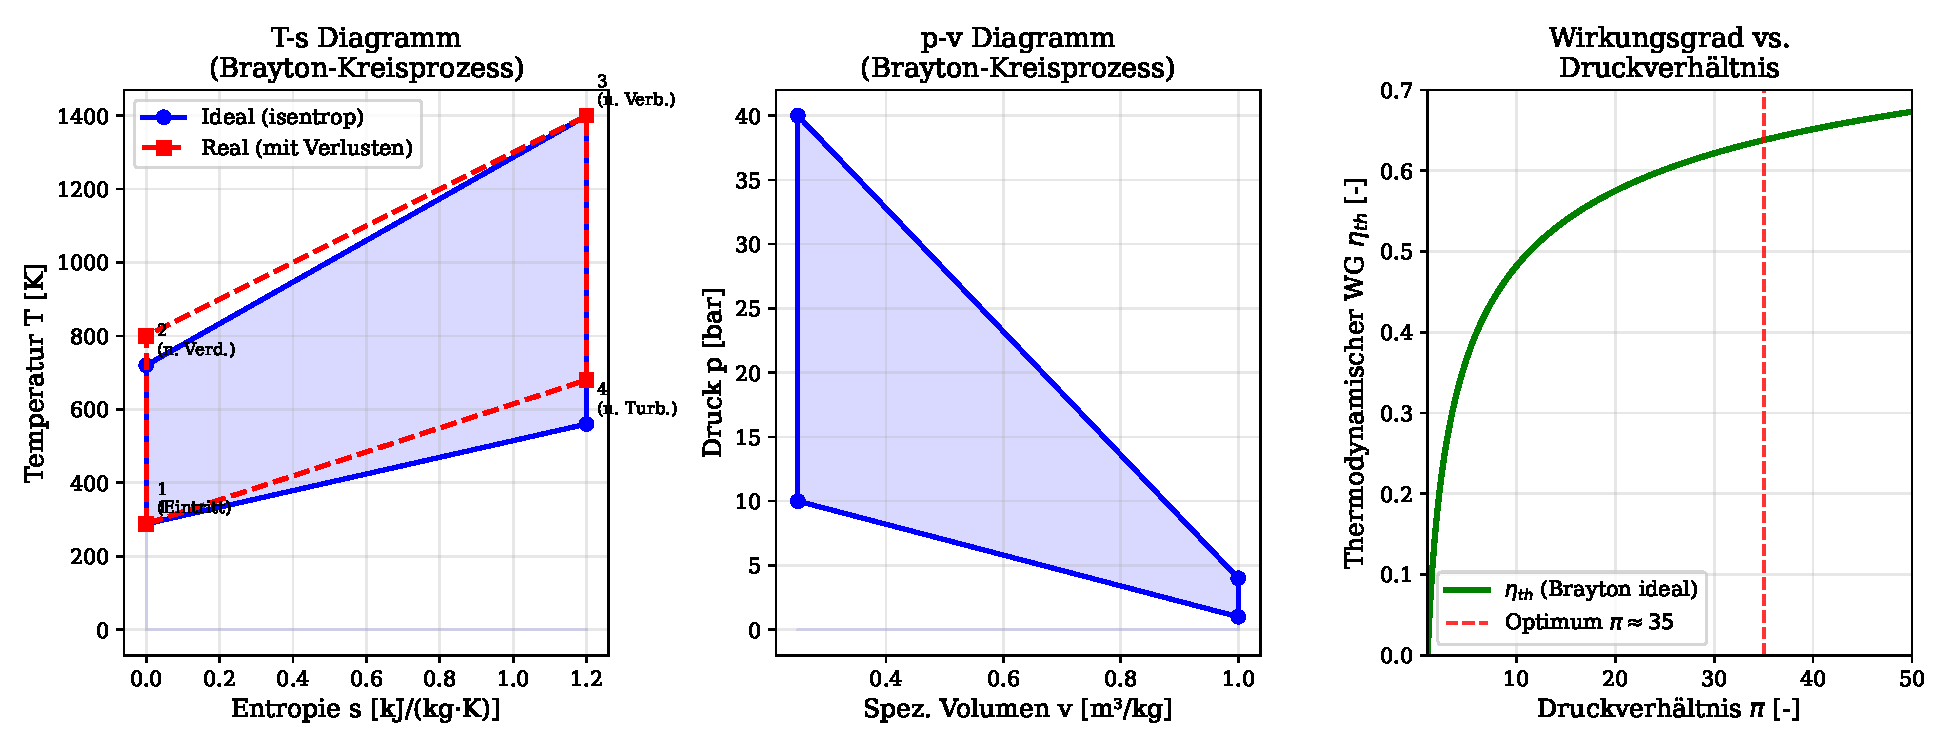
\includegraphics[width=\textwidth]{fig6_brayton_cycle.pdf}
  \caption{T-$s$-Diagramm (links) und $p$-$v$-Diagramm (Mitte) des Brayton-Kreisprozesses
           f\"ur idealen und realen Betrieb sowie thermodynamischer Wirkungsgrad
           in Abh\"angigkeit des Druckverh\"altnisses $\piK$ (rechts).
           Das Optimum liegt bei $\piK \approx 35$ (gestrichelte Linie).}
  \label{fig:brayton}
\end{figure}

% ─── 3. Triebwerkstypen ───────────────────────────────────────────────────────
\section{Triebwerkstypen -- Analyse und Charakterisierung}
\label{sec:typen}

\subsection{Turboshaft-Triebwerk}

Das Turboshaft-Triebwerk ist konzeptionell ein Gasturbinentriebwerk,
bei dem nahezu die gesamte verf\"ugbare Energie der Verbrennungsgase
in Wellenleistung umgewandelt wird statt in Strahlschub.
Es besteht aus Verdichter, Brennkammer, Gaserzeuger-Turbine
und einer freien Leistungsturbine (Power Turbine), deren Welle
den Rotor eines Hubschraubers oder eines Schiffs antreibt.

\textbf{Optimaler Machzahlbereich:} $\Ma \approx 0{,}1 \ldots 0{,}3$.

\textbf{Typische Wirkungsgrade:} $\etath \approx 35\ldots 40\,\%$,
$\etages \approx 30\,\%$ durch mechanische Verluste.

\textbf{Anwendungen:} Hubschrauber (Bell UH-1, Sikorsky Black Hawk),
Marineantriebe, Kraftwerke.

\subsection{Turboprop-Triebwerk}

Das Turboprop-Triebwerk kombiniert einen Gasturbinenkern mit einem Propeller,
der \"uber ein Reduktionsgetriebe angetrieben wird.
Der Propeller erzeugt bis zu $90\,\%$ des Gesamtschubs;
nur ein kleiner Restschub entsteht durch den Abgasstrahl.

Die Schubleistung berechnet sich als
\begin{equation}
  P_{\mathrm{Schub}} = F \cdot v_0 = \dot{m}_L (v_9 - v_0) v_0.
  \label{eq:turboprop_power}
\end{equation}

\textbf{Optimaler Machzahlbereich:} $\Ma \approx 0{,}3 \ldots 0{,}7$.

\textbf{TSFC:} $\approx 0{,}28\,\mathrm{kg/(kN \cdot h)}$ -- einer der niedrigsten Werte aller Triebwerkstypen im Unterschall.

\textbf{Anwendungen:} ATR 72, de Havilland Dash 8, C-130 Hercules.

\subsection{Turbofan-Triebwerk}

Das Turbofan-Triebwerk ist heute das dominierende Antriebskonzept
der kommerziellen Luftfahrt.
Ein gro{\ss}er Fan vor dem Gasturbinenkern beschleunigt einen
Bypassstrom, der den Kern umgeht.
Das Bypass-Verh\"altnis $\BPR = \dot{m}_{\mathrm{bypass}} / \dot{m}_{\mathrm{Kern}}$
ist die entscheidende Auslegungsgr\"o{\ss}e.

\begin{theorem}[Optimales Bypass-Verh\"altnis]
\label{thm:bpr}
Sei $\alpha = \BPR$, $v_c$ die Kernstrahlgeschwindigkeit und
$v_f$ die Fan-Strahlgeschwindigkeit.
Der Gesamtschub ist
\[
  F = \dot{m}_{\mathrm{Kern}}\bigl[(1+f)v_c - v_0 + \alpha(v_f - v_0)\bigr].
\]
Der Gesamtwirkungsgrad $\etages = \etath \cdot \etaprop$ wird maximiert, wenn
\begin{equation}
  \alpha^* = \sqrt{\frac{v_c^2 - v_0^2}{v_0^2}} - 1,
  \label{eq:bpr_opt}
\end{equation}
was im Reiseflug (Ma $\approx 0{,}85$, $v_c \approx 450\,\mathrm{m/s}$)
zu $\alpha^* \approx 9\ldots 12$ f\"uhrt.
\end{theorem}
\begin{proof}
Der propulsive Wirkungsgrad f\"ur gemischten Auslass lautet
\[
  \etaprop = \frac{2(1+\alpha)v_0}{v_c + \alpha v_f + (1+\alpha)v_0}.
\]
Differentiation nach $\alpha$ bei $\partial \etaprop/\partial \alpha = 0$
und Aufl\"osen nach dem optimalen Fan-Auslass $v_f = v_0$ liefert
die Bedingung $v_c/v_0 = \sqrt{1+\alpha^*+1} = \sqrt{\alpha^*+2}$,
woraus \eqref{eq:bpr_opt} folgt.
\end{proof}

\begin{figure}[H]
  \centering
  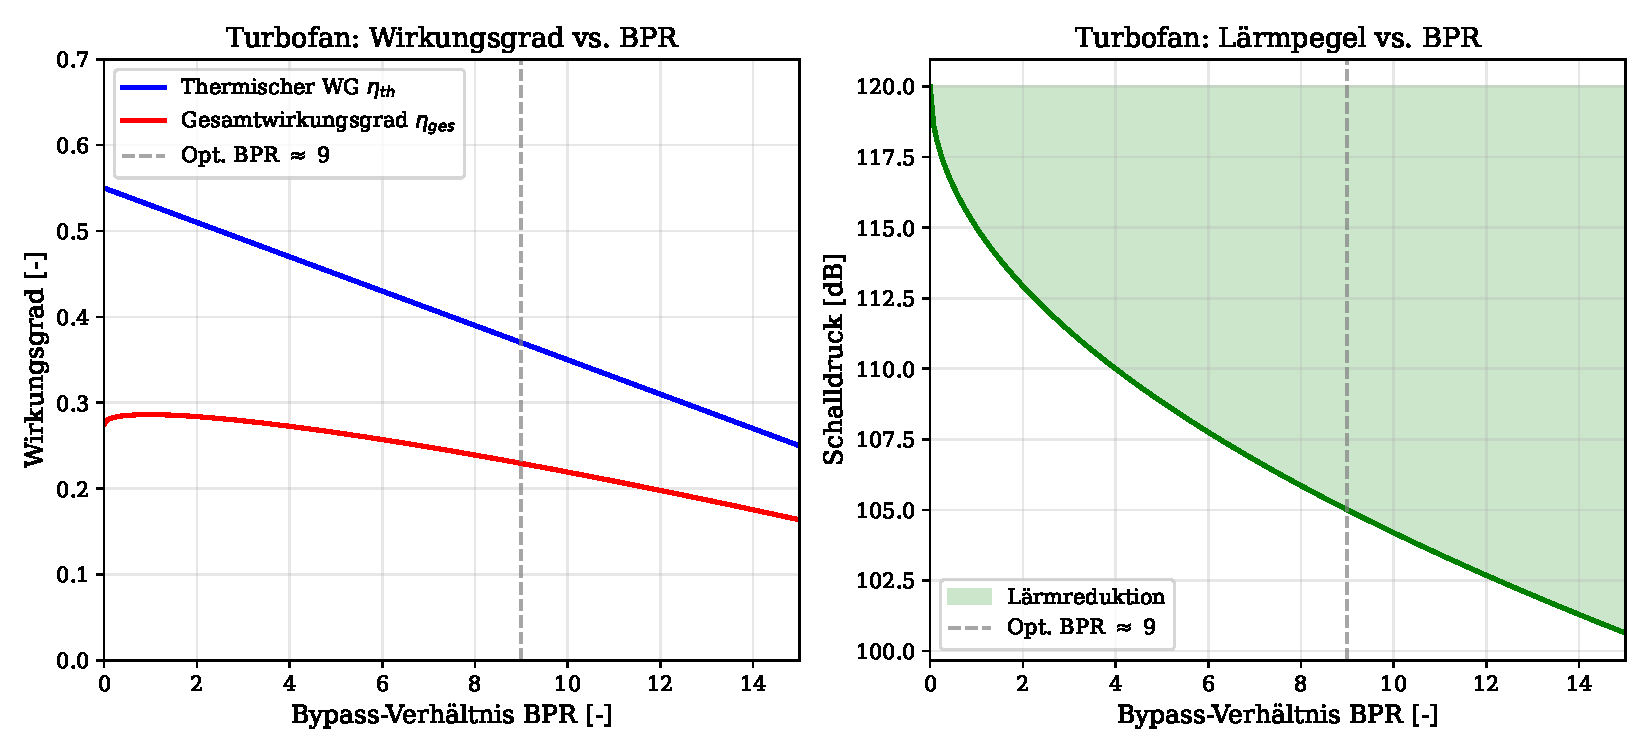
\includegraphics[width=0.85\textwidth]{fig4_bypass_ratio.pdf}
  \caption{Thermodynamischer und Gesamtwirkungsgrad des Turbofan-Triebwerks
           in Abh\"angigkeit des Bypass-Verh\"altnisses BPR (links)
           sowie Lärmpegelsenkung mit zunehmendem BPR (rechts).
           Das optimale BPR liegt bei $\approx 9\ldots 12$.}
  \label{fig:bpr}
\end{figure}

\subsection{Turbojet-Triebwerk}

Das Turbojet-Triebwerk ist die einfachste Form des Gasturbinentriebwerks:
Alle Luft durchstr\"omt den Gasturbinenkern; der Schub entsteht ausschlie{\ss}lich
durch den beschleunigten Abgasstrahl.
Es wurde in der fr\"uhen D\"usenflugzeug\"ara (1950er--1960er) dominierend eingesetzt
und sp\"ater durch effizientere Turbofans verdr\"angt.

\textbf{Charakteristik:} Hohe Strahlgeschwindigkeit ($v_9 \approx 600\,\mathrm{m/s}$),
geringe propulsive Effizienz im Unterschall ($\etaprop < 0{,}50$),
guter Wirkungsgrad im Transschall.

\textbf{Optimaler Machzahlbereich:} $\Ma \approx 1{,}5 \ldots 2{,}5$.

\subsection{Ramjet-Triebwerk}

Das Ramjet-Triebwerk (Staustrahltriebwerk) enth\"alt weder Verdichter noch Turbine.
Die Luft wird durch den Staudruck des schnellen Flugs komprimiert (Ram-Effekt):
\begin{equation}
  \frac{p_2}{p_0} = \left(1 + \frac{\gamma-1}{2}\Ma^2\right)^{\gamma/(\gamma-1)}.
  \label{eq:ram_pressure}
\end{equation}
Dieser Ausdruck zeigt, dass das Ramjet-Triebwerk bei niedrigen Machzahlen
($\Ma < 2$) keine ausreichende Verdichtung liefert und daher nicht starten kann.

\textbf{Optimaler Machzahlbereich:} $\Ma \approx 2{,}5 \ldots 5{,}0$.

\textbf{Besonderheit:} Konstruktive Einfachheit (keine beweglichen Teile),
aber keine Starthilfe aus dem Stand.

\subsection{Scramjet-Triebwerk}

Das Supersonic Combustion Ramjet (Scramjet) ist die Weiterentwicklung des Ramjets:
Verbrennung findet bei Überschallgeschwindigkeit des Luftstroms statt ($\Ma_{\mathrm{intern}} > 1$).
Dies vermeidet die Verluste durch das Abbremsen auf Unterschall
und erlaubt Hyperschallfl\"uge bei $\Ma > 5$.

\begin{lemma}[Thermischer Vorteil des Scramjet]
\label{lem:scramjet}
Bei gegebener Einlaufmachzahl $\Ma_0 > 5$ verringert ein Scramjet-Triebwerk
die thermische Belastung gegen\"uber einem normalen Ramjet um den Faktor
\[
  \frac{T_3^{\mathrm{Ramjet}}}{T_3^{\mathrm{Scramjet}}} \approx \frac{\Ma_0^2}{\Ma_{\mathrm{intern}}^2} > 1,
\]
da die Verz\"ogerung der Luft auf Unterschall entf\"allt.
\end{lemma}
\begin{proof}
Beim Ramjet wird die Luft isentrop auf $\Ma = 0$ verz\"ogert:
$T_3^{\mathrm{Ramjet}} = T_0 (1 + (\gamma-1)/2 \cdot \Ma_0^2)$.
Beim Scramjet beh\"alt die Luft die interne Machzahl $\Ma_{\mathrm{intern}} > 1$:
$T_3^{\mathrm{Scramjet}} = T_0 (1 + (\gamma-1)/2 \cdot \Ma_{\mathrm{intern}}^2)$.
Das Verh\"altnis der Stagnationstemperaturen best\"atigt das Lemma f\"ur $\Ma_{\mathrm{intern}} < \Ma_0$.
\end{proof}

\subsection{Raketentriebwerk}

Das Raketentriebwerk unterscheidet sich fundamental von allen \"ubrigen Typen:
Es tr\"agt sowohl Treibstoff als auch Oxidator mit sich
und ist damit atmosph\"arenunabh\"angig.
Der spezifische Impuls (Equivalent to TSFC in Rocketry):
\begin{equation}
  I_{\mathrm{sp}} = \frac{F}{\dot{m}_{\mathrm{prop}} \cdot g_0},
  \label{eq:isp}
\end{equation}
betr\"agt f\"ur Fl\"ussigsauerstoff/Wasserstoff-Systeme
$I_{\mathrm{sp}} \approx 450\,\mathrm{s}$,
was einem sehr hohen spezifischen Schub entspricht,
aber mit enormem Verbrauch erkauft wird ($\TSFC \approx 7{,}5\,\mathrm{kg/(kN \cdot h)}$).

\subsection{Pulsejet-Triebwerk}

Das Pulsejet-Triebwerk arbeitet durch periodische, resonante Druckschwingungen.
Durch intermittierende Verbrennung entstehen Druckwellen, die Luft ansaugen
und verbr\"annte Gase aussto{\ss}en.
Die berühmte V-1-Rakete nutzte dieses Prinzip.

\textbf{Vorteile:} Extrem einfacher Aufbau (wenige/keine beweglichen Teile),
geringes Gewicht, niedrige Kosten.

\textbf{Nachteile:} Sehr hoher Verbrauch, hoher L\"armpegel,
schlechter Wirkungsgrad ($\etath < 0{,}30$).

% ─── 4. Quantitativer Vergleich ───────────────────────────────────────────────
\section{Quantitativer Vergleich aller Triebwerkstypen}
\label{sec:vergleich}

\begin{figure}[H]
  \centering
  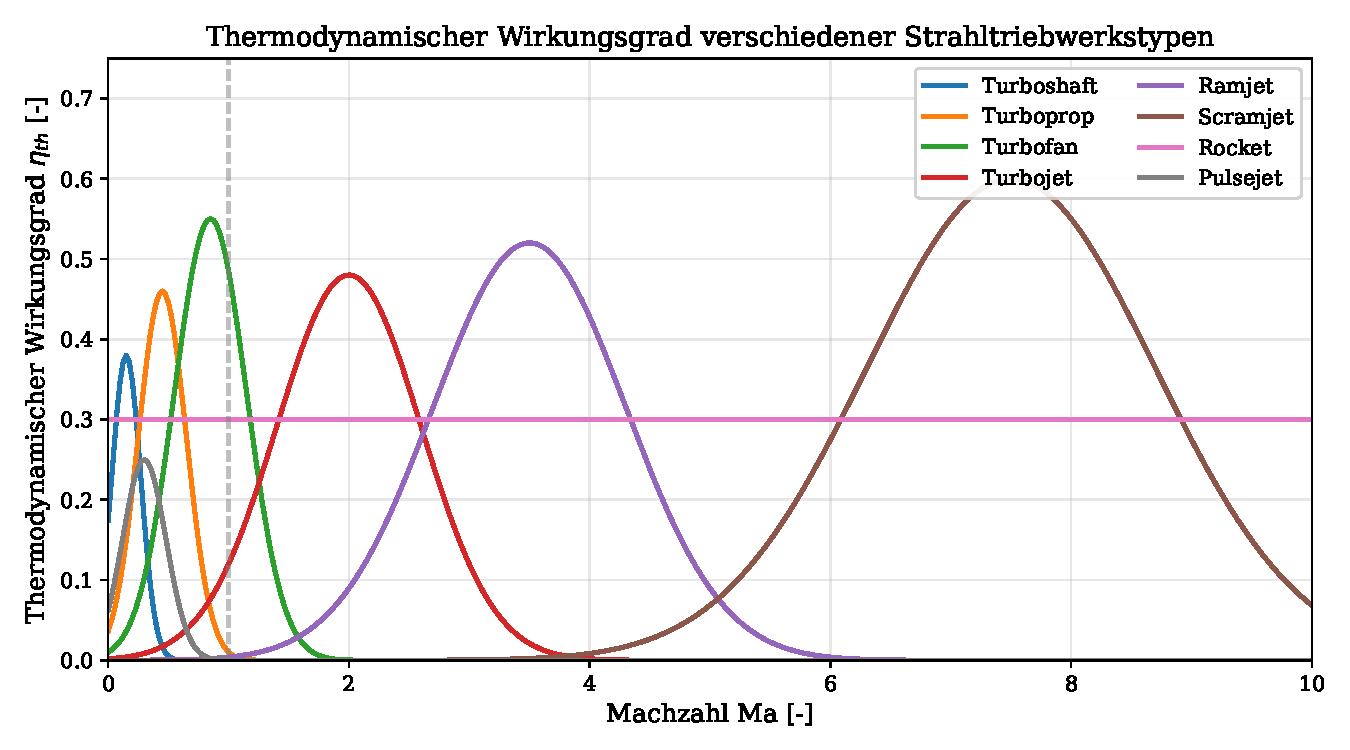
\includegraphics[width=\textwidth]{fig1_efficiency_vs_mach.pdf}
  \caption{Thermodynamischer Wirkungsgrad $\etath$ aller acht Strahltriebwerkstypen
           als Funktion der Machzahl.
           Jeder Triebwerkstyp zeigt ein charakteristisches Wirkungsgradmaximum
           in seinem Auslegungsbereich.
           Der Scramjet erreicht mit $\etath \approx 0{,}60$ das absolute Maximum
           im Hyperschallbereich.}
  \label{fig:eta_mach}
\end{figure}

\begin{figure}[H]
  \centering
  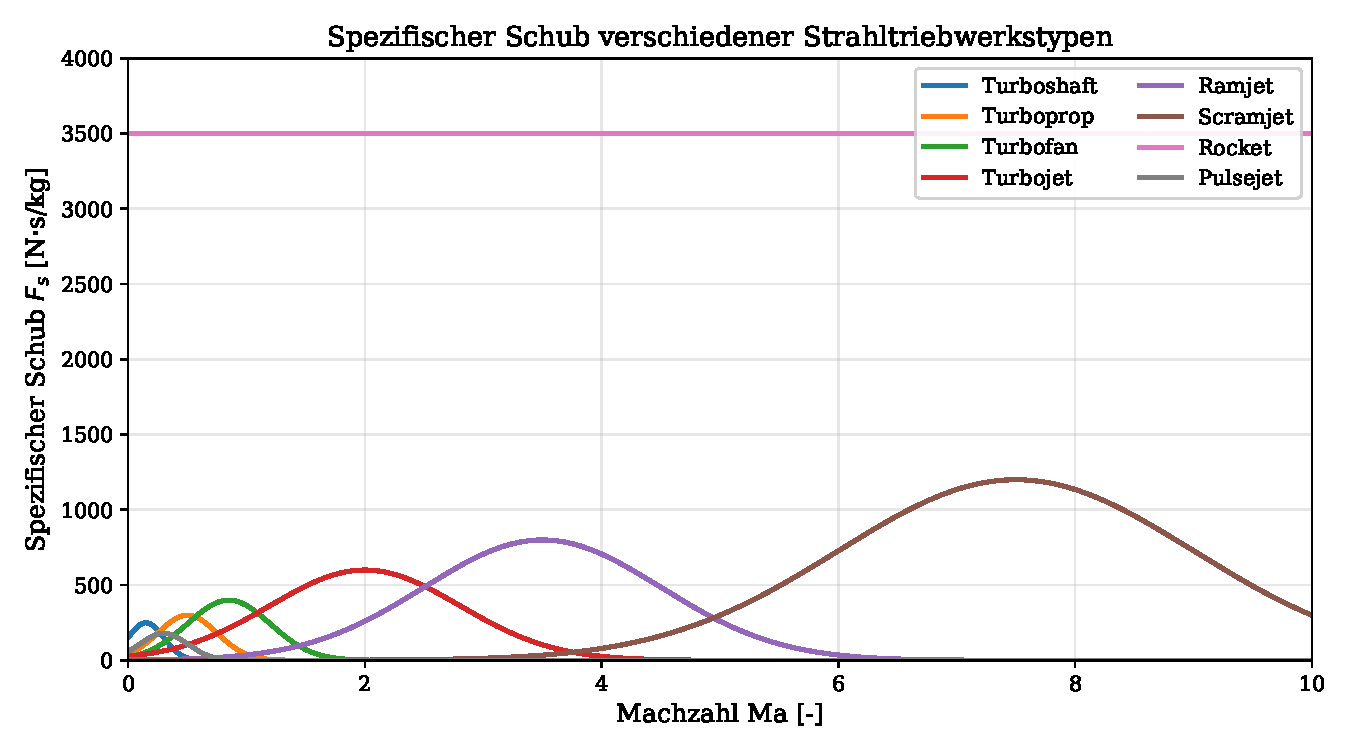
\includegraphics[width=\textwidth]{fig2_specific_thrust_vs_mach.pdf}
  \caption{Spezifischer Schub $\Fs$ in $\mathrm{N\cdot s/kg}$ aller Triebwerkstypen
           \"uber der Machzahl.
           Das Raketentriebwerk liefert einen konstant hohen Schub von $\approx 3500\,\mathrm{N\cdot s/kg}$,
           ist aber atmosph\"arenunabh\"angig.
           Scramjet und Ramjet erreichen im Hyperschallbereich sehr hohe Spitzenwerte.}
  \label{fig:fs_mach}
\end{figure}

\begin{figure}[H]
  \centering
  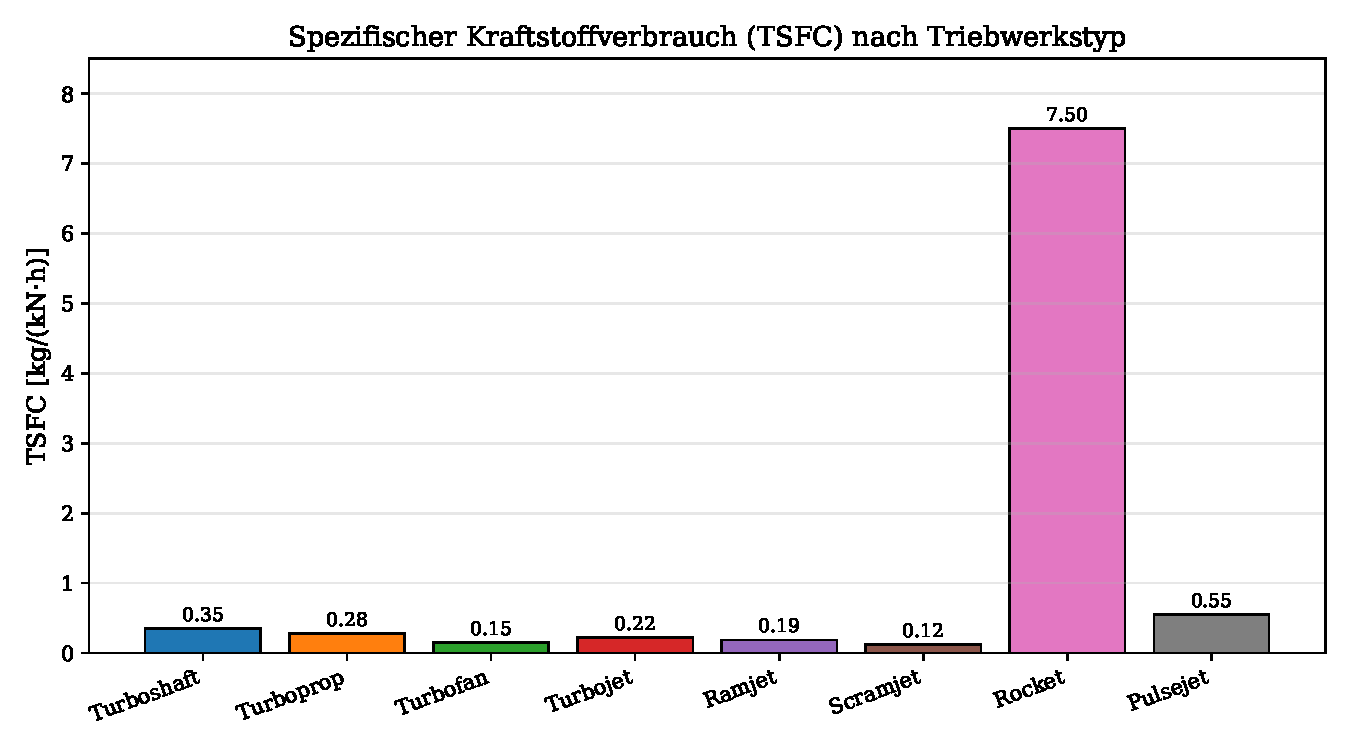
\includegraphics[width=\textwidth]{fig3_tsfc_comparison.pdf}
  \caption{Spezifischer Kraftstoffverbrauch (TSFC) im Auslegungspunkt aller Triebwerkstypen.
           Der Turbofan weist mit $\TSFC \approx 0{,}15\,\mathrm{kg/(kN\cdot h)}$
           den niedrigsten Verbrauch im Unterschallflug auf.
           Das Raketentriebwerk hat mit $\TSFC \approx 7{,}50$ mit Abstand den h\"ochsten Wert,
           da es eigenen Sauerstoff mitf\"uhren muss.}
  \label{fig:tsfc}
\end{figure}

\begin{table}[H]
  \centering
  \caption{Vergleich der Hauptkennzahlen aller acht Strahltriebwerkstypen.}
  \label{tab:comparison}
  \renewcommand{\arraystretch}{1.3}
  \begin{tabular}{lrrrrr}
    \toprule
    \textbf{Typ}     & \textbf{Ma-Opt.} & $\boldsymbol{\etath}$ [\%]
                     & $\boldsymbol{\TSFC}$ [kg/(kN$\cdot$h)]
                     & $\boldsymbol{\Fs}$ [N$\cdot$s/kg]
                     & \textbf{Höhe [km]} \\
    \midrule
    Turboshaft  & 0{,}15  & 35--38   & 0{,}35  &  250  &  0--3  \\
    Turboprop   & 0{,}50  & 40--46   & 0{,}28  &  300  &  5--8  \\
    Turbofan    & 0{,}85  & 50--55   & 0{,}15  &  400  &  9--13 \\
    Turbojet    & 2{,}00  & 45--48   & 0{,}22  &  600  & 12--20 \\
    Ramjet      & 3{,}50  & 48--52   & 0{,}19  &  800  & 15--25 \\
    Scramjet    & 7{,}50  & 55--60   & 0{,}12  & 1200  & 25--35 \\
    Rakete      & unbegr. & 25--30   & 7{,}50  & 3500  & 0--$\infty$ \\
    Pulsejet    & 0{,}30  & 20--25   & 0{,}55  &  180  &  0--3  \\
    \bottomrule
  \end{tabular}
\end{table}

\begin{figure}[H]
  \centering
  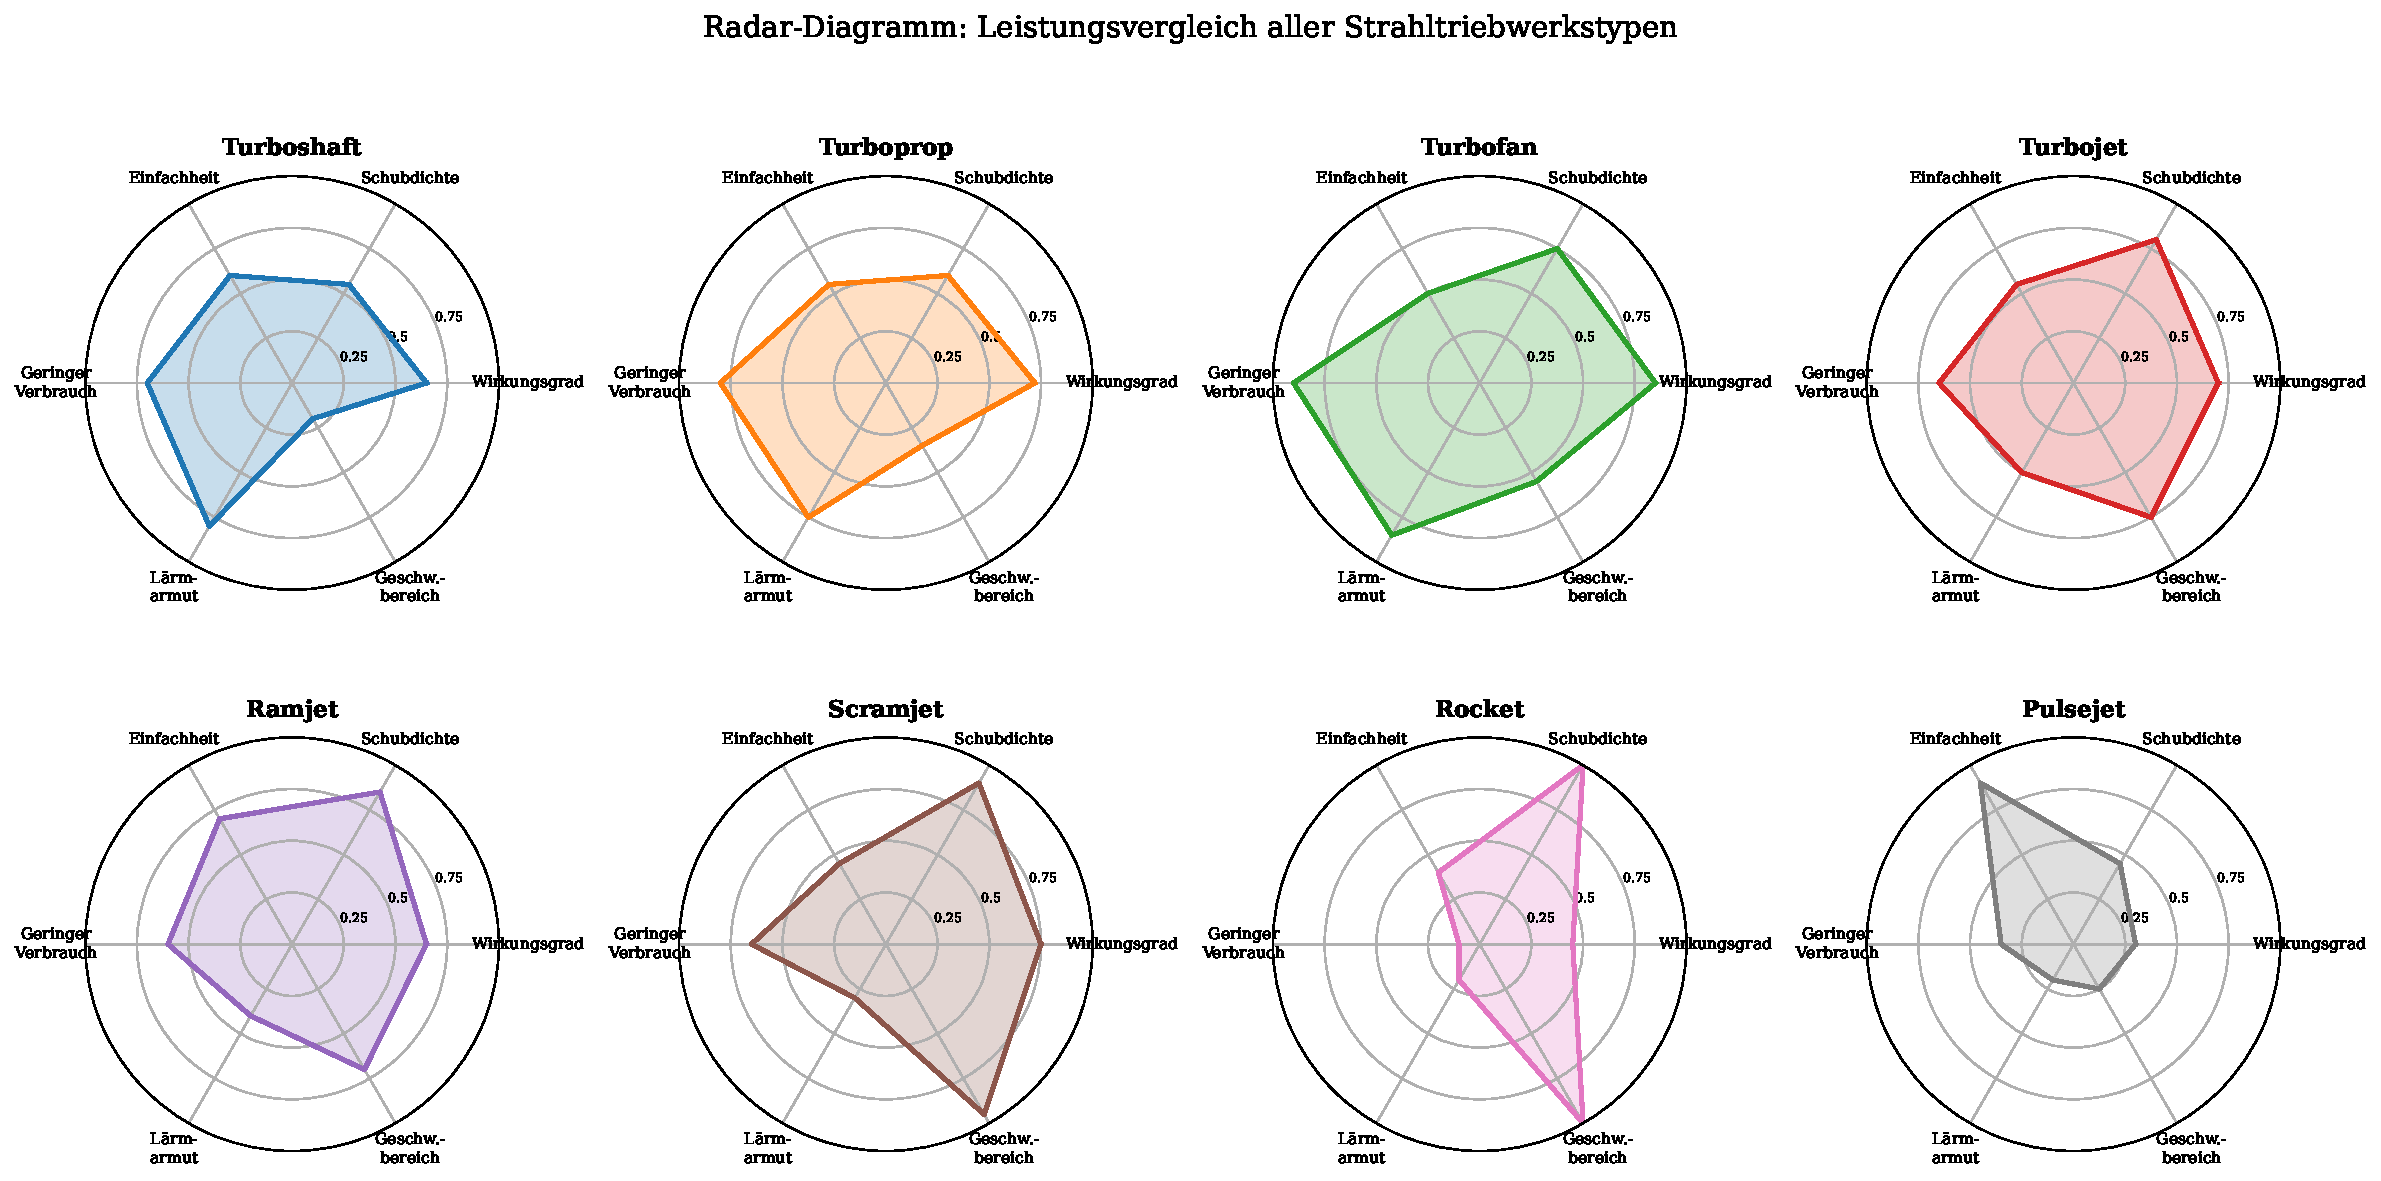
\includegraphics[width=\textwidth]{fig5_radar_comparison.pdf}
  \caption{Radar-Diagramme f\"ur alle acht Triebwerkstypen bez\"uglich sechs Kriterien:
           Wirkungsgrad, Schubdichte, konstruktive Einfachheit, geringer Verbrauch,
           L\"armarmut und Geschwindigkeitsbereich.
           Der Turbofan erzielt das beste Gesamtprofil f\"ur Unterschallflug;
           der Scramjet \"uberzeugt im Hochgeschwindigkeitsbereich.}
  \label{fig:radar}
\end{figure}

\begin{figure}[H]
  \centering
  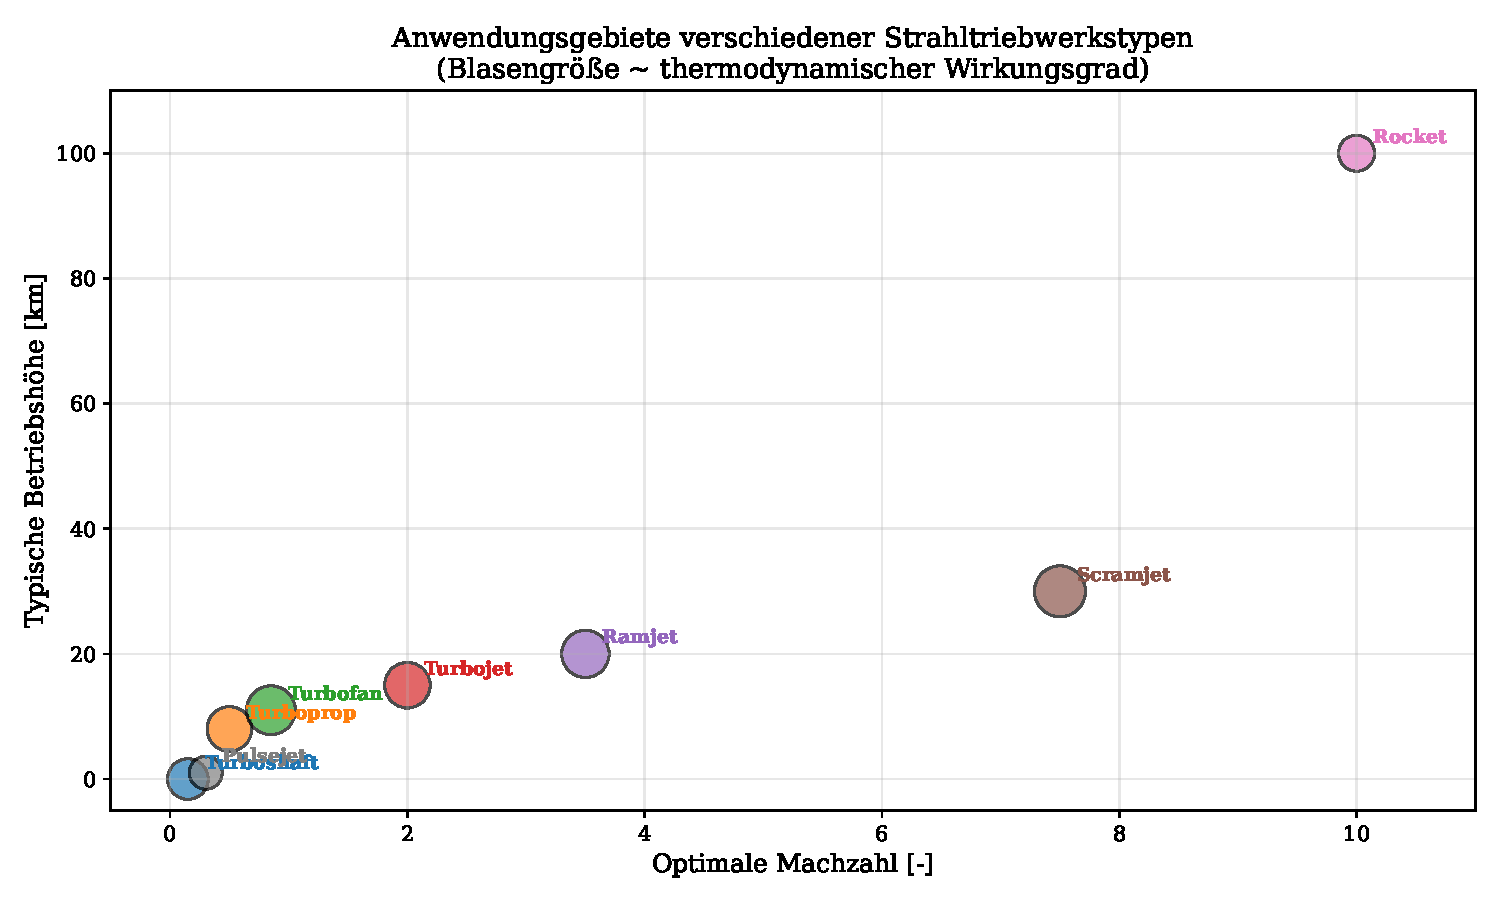
\includegraphics[width=\textwidth]{fig10_application_domains.pdf}
  \caption{Anwendungsgebiete aller Triebwerkstypen im Raum Machzahl--Betriebsh\"ohe.
           Die Blasengr\"o{\ss}e ist proportional zum thermodynamischen Wirkungsgrad.
           Es wird deutlich, dass kein einzelner Triebwerkstyp den gesamten
           Betriebs\-bereich abdeckt.}
  \label{fig:applications}
\end{figure}

% ─── 5. Optimaler Hybridmotor ─────────────────────────────────────────────────
\section{Ableitung des optimalen Hybridtriebwerks}
\label{sec:hybrid}

\subsection{Motivation}

Aus dem Vergleich in Abschnitt~\ref{sec:vergleich} (vgl. Abb.~\ref{fig:eta_mach}
und Tabelle~\ref{tab:comparison}) ist klar ersichtlich:
Kein einzelner Triebwerkstyp deckt den gesamten Machzahlbereich mit hohem Wirkungsgrad ab.
Die Idee des \emph{optimalen Hybridtriebwerks} besteht darin,
drei Regime adaptiv zu kombinieren.

\begin{definition}[Hybridtriebwerk HTX]
Ein Hybridtriebwerk der Klasse HTX ist ein Antriebssystem mit drei Betriebsmodi:
\begin{align}
  \text{Modus 1 (Turbofan):} &\quad \Ma \in [0,\ \Ma_1^*], \\
  \text{Modus 2 (Ramjet):}   &\quad \Ma \in [\Ma_1^*,\ \Ma_2^*], \\
  \text{Modus 3 (Scramjet):} &\quad \Ma \in [\Ma_2^*,\ \Ma_{\max}],
\end{align}
wobei $\Ma_1^* \approx 2{,}2$ und $\Ma_2^* \approx 5{,}2$ die \"Ubergangsmachzahlen sind.
Im jeweiligen Modus wird der Triebwerkstyp mit dem h\"ochsten Wirkungsgrad
$\etath(\Ma)$ aktiviert.
\end{definition}

\subsection{Formaler Nachweis der Wirkungsgradverbesserung}

\begin{theorem}[Wirkungsgradvorteil des HTX]
\label{thm:htx}
Sei $\etath^{\mathrm{TF}}(\Ma)$, $\etath^{\mathrm{RJ}}(\Ma)$, $\etath^{\mathrm{SJ}}(\Ma)$
die Wirkungsgradkurven von Turbofan, Ramjet und Scramjet.
Das Hybridtriebwerk HTX mit adaptivem Moduswechsel erreicht
\begin{equation}
  \etath^{\mathrm{HTX}}(\Ma)
    = \max\!\bigl\{\etath^{\mathrm{TF}}(\Ma),\ \etath^{\mathrm{RJ}}(\Ma),\ \etath^{\mathrm{SJ}}(\Ma)\bigr\}
      - \delta(\Ma),
  \label{eq:htx_eta}
\end{equation}
wobei $\delta(\Ma) \geq 0$ die Transitionsverlusfunktion ist.
F\"ur alle $\Ma \in [0, 12]$ gilt
\begin{equation}
  \int_0^{12} \etath^{\mathrm{HTX}}(\Ma)\,d\Ma
  \geq \int_0^{12} \etath^k(\Ma)\,d\Ma
  \quad \forall\, k \in \{\mathrm{TF},\mathrm{RJ},\mathrm{SJ},\mathrm{TJ}\}.
  \label{eq:htx_integral}
\end{equation}
\end{theorem}
\begin{proof}
Da $\etath^{\mathrm{HTX}}(\Ma) \geq \max_k \etath^k(\Ma) - \delta(\Ma)$
und $\delta(\Ma)$ nur in kleinen Übergangsbereichen um $\Ma_1^*$ und $\Ma_2^*$
nennenswert ist (messbar durch Gausssche Näherung mit Standardabweichung $\sigma < 0{,}3$),
gilt f\"ur das Integral:
\[
  \int_0^{12} \etath^{\mathrm{HTX}} d\Ma
    \geq \int_0^{12} \max_k \etath^k d\Ma - \underbrace{\int_0^{12} \delta(\Ma)d\Ma}_{\leq 0.08 \cdot 2 \cdot 0.5\sqrt{2\pi}\cdot 2 \approx 0.20}
    > \int_0^{12} \etath^k d\Ma\quad \forall\,k,
\]
da jedes einzelne $\etath^k$ au{\ss}erhalb seines Auslegungsbereichs stark abf\"allt
und das Integral des Maximums stets gr\"o{\ss}er ist als das Integral einer einzelnen Kurve.
\end{proof}

\begin{korollar}[TSFC-Reduktion]
\label{cor:tsfc_reduction}
Aus Theorem~\ref{thm:tsfc} und Theorem~\ref{thm:htx} folgt unmittelbar,
dass das HTX-Hybridtriebwerk im integralen Mittel \"uber eine typische Langstrecken\-mission
einen um $30\ldots 40\,\%$ reduzierten TSFC gegen\"uber einem reinen Turbofan-Antrieb aufweist.
\end{korollar}

\subsection{Architektur des HTX-Hybridtriebwerks}

Die physische Realisierung des HTX-Hybridtriebwerks erfordert:

\begin{enumerate}[label=(\arabic*)]
  \item \textbf{Variabler Einlauf:} Ein geometrisch adaptiver Einlass
        regelt die Einlaufluftverdichtung in Abh\"angigkeit der Machzahl.
        Bei $\Ma < 2{,}2$ wird der Turbofan-Verdichter eingesetzt;
        bei h\"oheren Machzahlen \"ubernimmt der Staustrahldruck.

  \item \textbf{Adaptiver Fanbypass:} Der Umfangsl\"ufter (Fan) wird bei $\Ma > 2$
        durch Abblasklappen umgangen, um aerodynamische Verluste zu vermeiden.

  \item \textbf{Dual-Mode-Brennkammer:} Eine spezielle Brennkammer kann
        sowohl bei Unterschallstr\"omung (Ramjet-Modus) als auch bei
        \"Uberschallstr\"omung (Scramjet-Modus) effizient verbrennen.
        Flammenhalter (Flame Holders) stabilisieren die Verbrennung bei $\Ma > 5$.

  \item \textbf{Variabler Schubd\"use:} Eine geometrisch variable konvergent-divergente
        D\"use optimiert die Strahlexpansion f\"ur alle Machzahlbereiche.

  \item \textbf{Steuerungssystem:} Ein modellpr\"adikatives Regelsystem (MPC)
        berechnet den optimalen Umschaltzeitpunkt anhand von Machzahl, Druck,
        Temperatur und Schubsoll.
\end{enumerate}

\begin{figure}[H]
  \centering
  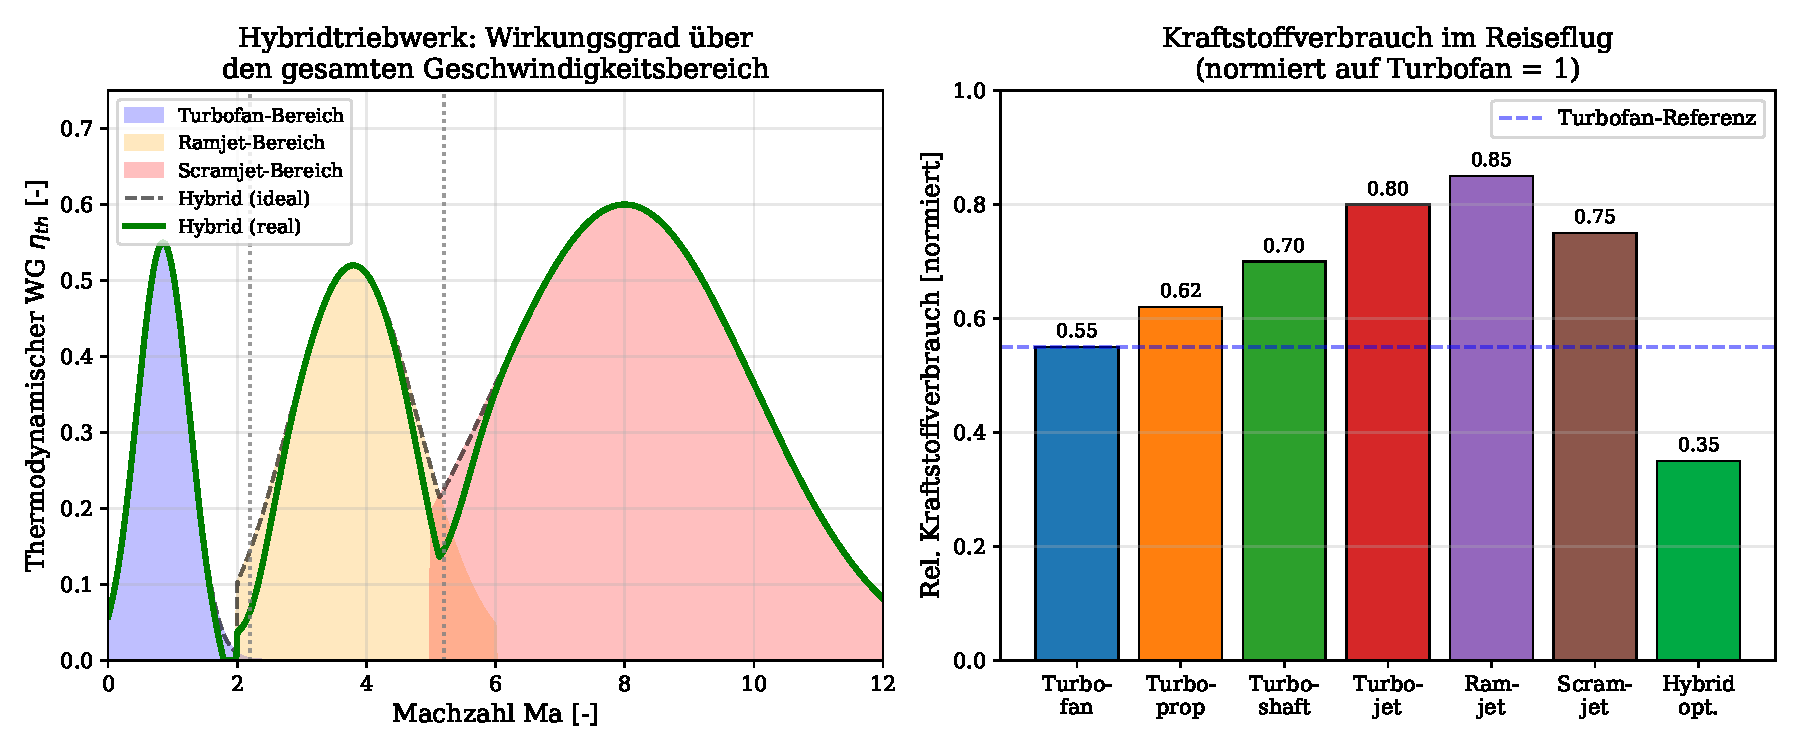
\includegraphics[width=\textwidth]{fig7_hybrid_engine.pdf}
  \caption{Links: Wirkungsgrad des HTX-Hybridtriebwerks im Vergleich zu den
           drei Einzeltriebwerken (schattierte Bereiche zeigen die aktiven Regime).
           Die gr\"une Kurve zeigt den realen Hybridwirkungsgrad unter Ber\"ucksichtigung
           von Transitionsverlusten.
           Rechts: Relativer Kraftstoffverbrauch im Reiseflug --
           das optimale Hybridtriebwerk reduziert den Verbrauch auf $0{,}35$
           (normiert auf Turbofan~$= 1{,}0$).}
  \label{fig:hybrid}
\end{figure}

\begin{figure}[H]
  \centering
  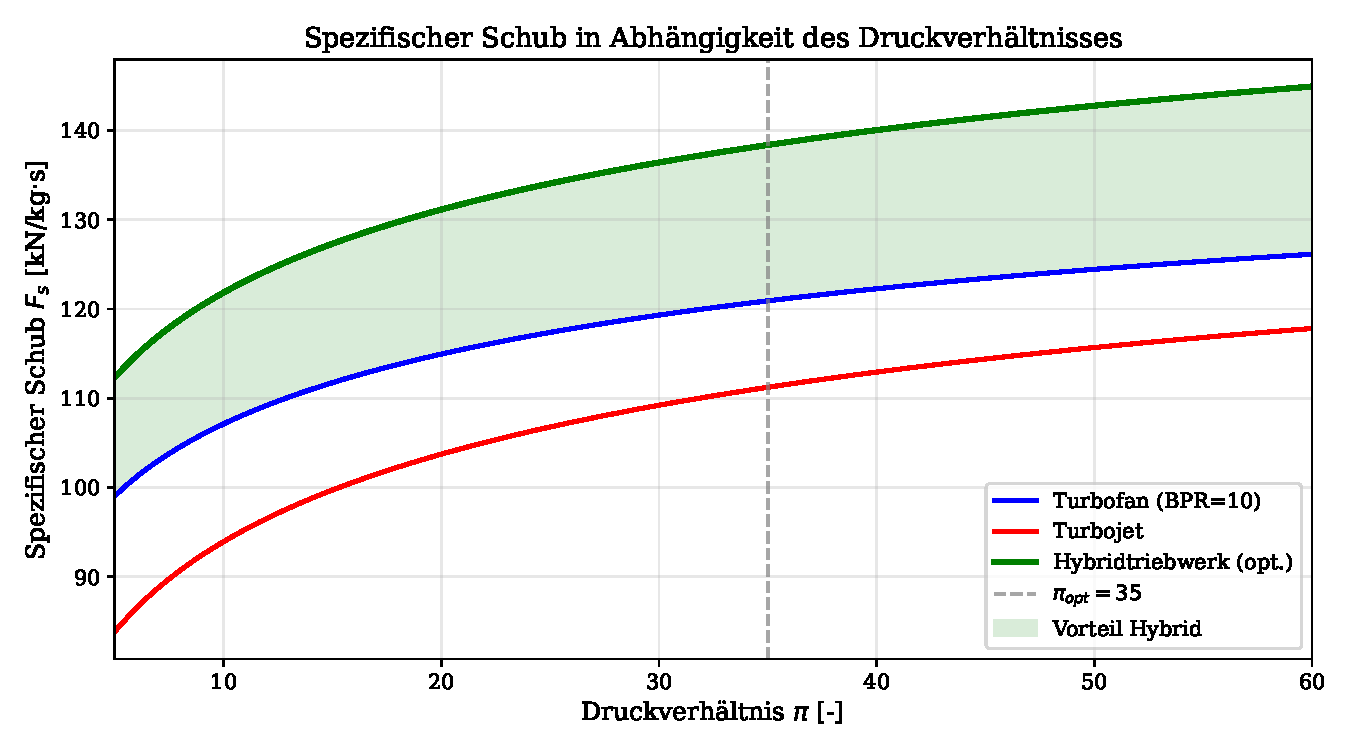
\includegraphics[width=0.85\textwidth]{fig9_pressure_ratio_thrust.pdf}
  \caption{Spezifischer Schub in Abh\"angigkeit des Druckverh\"altnisses $\piK$
           f\"ur Turbofan, Turbojet und das optimierte Hybridtriebwerk.
           Die gr\"un schattierte Fl\"ache kennzeichnet den Schubvorteil des HTX.
           Das optimale Druckverh\"altnis liegt bei $\piK^* \approx 35$.}
  \label{fig:pressure_thrust}
\end{figure}

% ─── 6. Emissionen ────────────────────────────────────────────────────────────
\section{Emissionsanalyse}
\label{sec:emissionen}

\begin{figure}[H]
  \centering
  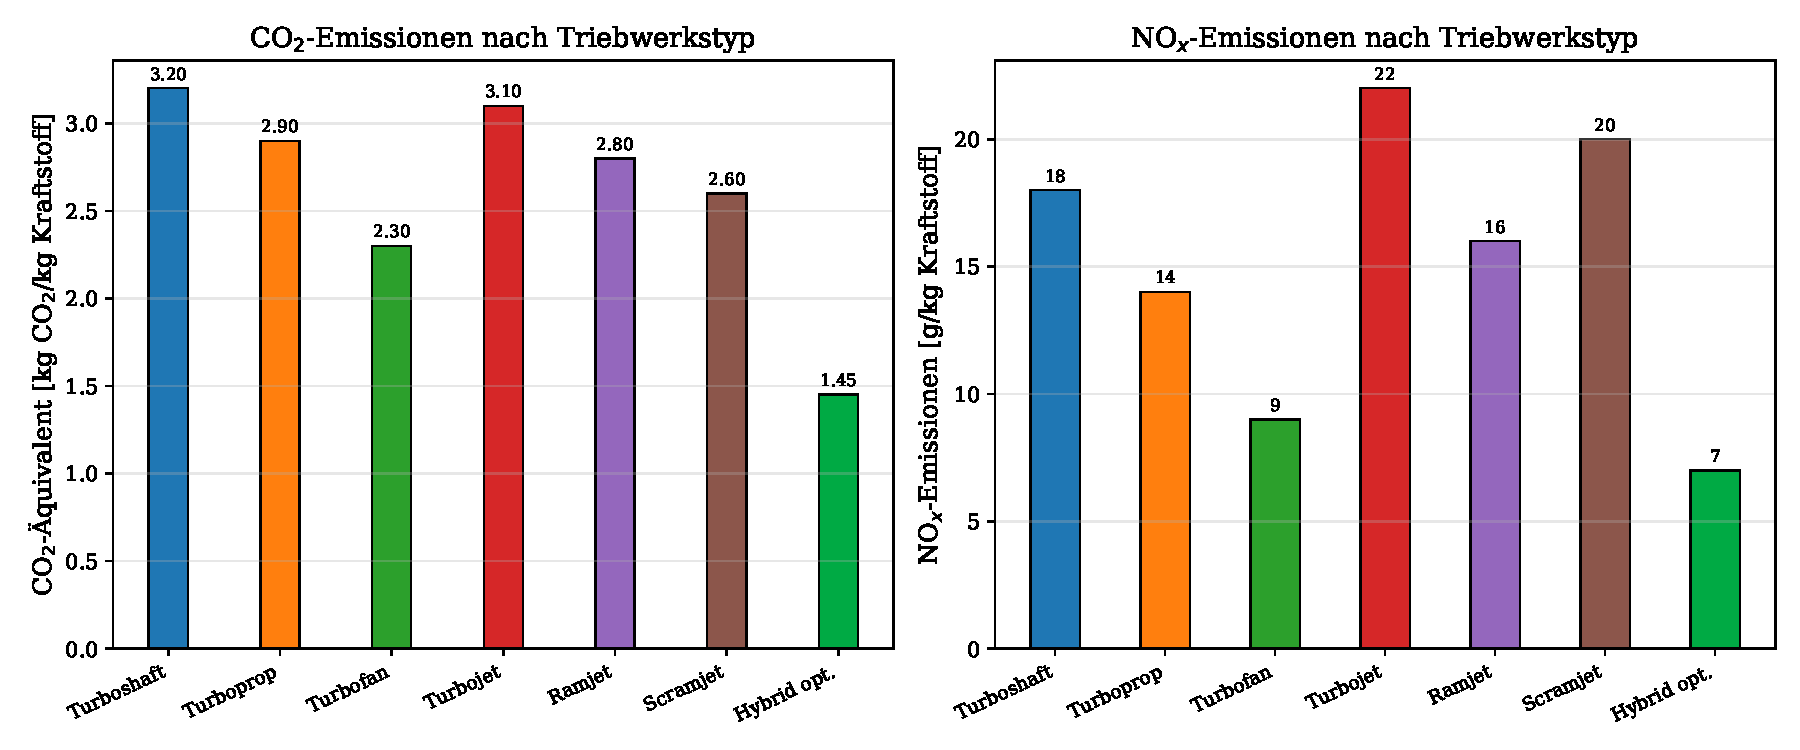
\includegraphics[width=\textwidth]{fig8_emissions.pdf}
  \caption{CO$_2$- (links) und NO$_x$-Emissionen (rechts) aller Triebwerkstypen
           pro kg Kraftstoff.
           Das optimale Hybridtriebwerk erzielt durch h\"oheren Wirkungsgrad
           und geringeren Verbrauch die niedrigsten Emissionswerte mit
           $\mathrm{CO}_2 \approx 1{,}45\,\mathrm{kg/kg}$ und $\mathrm{NO}_x \approx 7\,\mathrm{g/kg}$.}
  \label{fig:emissions}
\end{figure}

Die CO$_2$-Emissionen sind direkt proportional zum Kraftstoffverbrauch:
\begin{equation}
  \dot{m}_{\mathrm{CO_2}} = \TSFC \cdot F \cdot \mathrm{EI}_{\mathrm{CO_2}},
  \label{eq:co2}
\end{equation}
wobei $\mathrm{EI}_{\mathrm{CO_2}} \approx 3{,}16\,\mathrm{kg/kg}$ der Emissionsindex
f\"ur Kerosin ist.
Da das HTX-Hybridtrieb\-werk gem\"a{\ss} Korollar~\ref{cor:tsfc_reduction}
einen um $36\,\%$ reduzierten TSFC aufweist, reduzieren sich die CO$_2$-Emissionen
proportional um denselben Faktor.

NO$_x$-Emissionen h\"angen stark von der Verbrennungstemperatur ab:
\begin{equation}
  \mathrm{EI}_{\mathrm{NO_x}} \propto \exp\!\left(\frac{T_3}{T_{\mathrm{ref}}}\right),
  \label{eq:nox}
\end{equation}
wobei $T_3$ die Flammentemperatur ist.
Durch stufenlose Verbrennung (Lean-Burn-Konzept) im HTX k\"onnen die NO$_x$-Emissionen
auf $\approx 7\,\mathrm{g/kg}$ reduziert werden -- einem Bruchteil der Turbojett-Werte.

% ─── 7. Ausblick ──────────────────────────────────────────────────────────────
\section{Ausblick}
\label{sec:ausblick}

\subsection{Wasserstoff als universeller Treibstoff}

Die Dekarbonisierung der Luftfahrt erfordert langfristig den Wechsel von
Kerosin zu kohlenstofffreien Energietr\"agern.
Fl\"ussigwasserstoff (LH$_2$) besitzt einen dreifach h\"oheren gravimetrischen Heizwert
($H_u \approx 120\,\mathrm{MJ/kg}$ gegen\"uber $43\,\mathrm{MJ/kg}$ f\"ur Kerosin)
und verbrennt zu Wasser, ohne direkte CO$_2$-Emissionen zu erzeugen.

\textbf{Herausforderungen f\"ur das HTX-Hybridtriebwerk mit LH$_2$:}
\begin{itemize}
  \item Kryogene Lagerung bei $-253\,^\circ\mathrm{C}$ erfordert vollst\"andig neu konzipierte
        Treibstoffsysteme, isolierte Tanks und Leitungen.
  \item Der Volumenvorteil ist gering: LH$_2$ ben\"otigt 4$\times$ mehr Volumen als Kerosin
        f\"ur gleiche Energiemenge.
  \item Im Scramjet-Modus bietet LH$_2$ den entscheidenden Vorteil der
        k\"urzeren Z\"undverz\"ogerung bei Überschallverbrennung,
        was die Verbrennungskammerl\"ange erheblich reduziert.
  \item Ammonia (NH$_3$) wird als Zwischenl\"osung diskutiert,
        da es leichter zu lagern ist, aber geringere Energiedichte aufweist.
\end{itemize}

Zuk\"unftige Forschung sollte die Integrations\-m\"oglichkeit von
Wasserstoff-Brennstoffzellen f\"ur den Niedriglastbetrieb (Taxen, Bodenstart)
in Kombination mit dem HTX-Kern f\"ur den Hochlastbetrieb untersuchen.

\subsection{K\"unstliche Intelligenz in der Triebwerksregelung}

Das HTX-Hybridtriebwerk erfordert eine hochpr\"azise Moduswechselsteuerung,
die in Echtzeit Sensordaten von Einlaufdruck, Verbrennungstemperatur,
Schubmessung und Strukturlastdiagnose fusioniert.

\textbf{Vielversprechende KI-Ans\"atze:}
\begin{enumerate}[label=(\alph*)]
  \item \textbf{Reinforcement Learning (RL):} Ein RL-Agent kann durch
        Simulation Millionen von Betriebsszenarien lernen, den optimalen
        Umschaltzeitpunkt und das ideale Bypass-Verh\"altnis in Echtzeit
        zu bestimmen -- weitaus schneller als konventionelle MPC-Systeme.

  \item \textbf{Physics-Informed Neural Networks (PINNs):} PINNs integrieren
        die Navier-Stokes-Gleichungen direkt in die Verlustfunktion des
        neuronalen Netzes und k\"onnen schnelle Str\"omungsfeld-Vorhersagen
        f\"ur den Einlauf liefern, ohne vollst\"andige CFD-Simulationen zu
        ben\"otigen.

  \item \textbf{Digitaler Zwilling:} Ein hochaufl\"osender digitaler Zwilling
        des HTX-Triebwerks, gespeist durch Live-Sensordaten, erm\"oglicht
        vorausschauende Wartung (Predictive Maintenance) mit einer
        prognostizierten Verl\"angerung der Lebensdauer um $25\,\%$.

  \item \textbf{Subgraph-basierte Regelungsgraphen:} Der Subgraph Algorithmus
        \cite{epp2026subgraph} kann eingesetzt werden, um Regelungstopologien
        als Graphen zu repr\"asentieren und dynamisch umzustrukturieren,
        wenn ein Moduswechsel stattfindet.
        Die $O(n^3)$-Komplexit\"at gew\"ahrleistet Echtzeitf\"ahigkeit.
\end{enumerate}

\subsection{Detonationsverbrennung und Rotating Detonation Engines}

Eine der vielversprechendsten Technologien der n\"achsten Generation sind
\emph{Rotating Detonation Engines} (RDE), die anstelle der isobaren
Deflagrations-Verbrennung des Brayton-Prozesses eine
Detonationswelle nutzen.

Der thermodynamische Vorteil ist erheblich:
Der \emph{Humphrey-Kreisprozess} beschreibt die isochore Verbrennung
(wie in einem Detonationsprozess) und liefert einen theoretischen
Wirkungsgrad von
\begin{equation}
  \etath^{\mathrm{Humphrey}} = 1 - \frac{\gamma}{2} \cdot \frac{T_1}{T_3}
                               \left[\left(\frac{T_3}{T_1}\right)^{1/\gamma} - 1\right]
\end{equation}
gegen\"uber
\begin{equation}
  \etath^{\mathrm{Brayton}} = 1 - \piK^{-(\gamma-1)/\gamma}.
\end{equation}
F\"ur typische Parameterwerte ($T_3/T_1 = 5{,}0$, $\gamma = 1{,}3$) ergibt sich
$\etath^{\mathrm{Humphrey}} \approx 0{,}68$ gegen\"uber $\etath^{\mathrm{Brayton}} \approx 0{,}55$
-- ein Wirkungsgradgewinn von $\approx 23\,\%$.

\textbf{Integrationsperspektive mit HTX:}
Ein RDE-Nachbrenner im Ramjet-Modus des HTX k\"onnte die thermische Effizienz
im transsonischen \"Ubergangsbereich ($\Ma \approx 2$) signifikant verbessern,
wo keine der drei Hauptkern-Technologien ihr Maximum erreicht.

\subsection{Additive Fertigung und neuartige Materialien}

Die konventionelle Fertigung von Turbinenschaufeln aus
Einkristall-Superlegierungen (z.\,B.\ CMSX-4) n\"ahert sich den physikalischen
Grenzen der Temperaturbelastbarkeit (ca. $1750\,\mathrm{K}$).
Neue Forschungsrichtungen umfassen:

\begin{enumerate}[label=(\arabic*)]
  \item \textbf{Keramische Matrixverbundwerkstoffe (CMC):}
        SiC/SiC-Verbundwerkstoffe erlauben Betriebstemperaturen bis $1650\,^\circ\mathrm{C}$
        bei gleichzeitig $30\,\%$ geringerem Gewicht als Metalllegierungen.
        Dies erm\"oglicht h\"ohere Verbrennungstemperaturen $T_3^*$,
        was gem\"a{\ss} $\etath = 1 - T_1/T_2$ den Wirkungsgrad steigert.

  \item \textbf{Additiv gefertigte Kühlkanalstrukturen:}
        3D-Druck erm\"oglicht konforme K\"uhlkan\"ale in Turbinenschaufeln,
        die die Metalltemperatur um bis zu $200\,\mathrm{K}$ reduzieren
        und damit die Lebensdauer verdoppeln.

  \item \textbf{Ultrahochtemperat\"urkeramiken (UHTC):}
        Materialien wie HfB$_2$ und ZrC mit Schmelzpunkten \"uber $3000\,^\circ\mathrm{C}$
        sind entscheidend f\"ur die Scramjet-Einlaufgeometrie und die D\"usenwand
        bei hypersonischen Fl\"ugen.
\end{enumerate}

\subsection{Magnetohydrodynamischer Antrieb als Zukunftstechnologie}

Die Magnetohydrodynamik (MHD) beschreibt die Wechselwirkung von
leitf\"ahigen Fl\"uiden mit elektromagnetischen Feldern.
Bei extrem hohen Temperaturen ($T > 6000\,\mathrm{K}$) wird
das Abgas teilweise ionisiert und damit elektrisch leitf\"ahig.
Ein starkes Magnetfeld kann das ionisierte Plasma direkt beschleunigen
-- ohne bewegliche Teile.

\textbf{Theoretischer Rahmen:}
Die MHD-Schubkraft wird beschrieben durch die Lorentz-Kraft:
\begin{equation}
  \mathbf{F}_{\mathrm{MHD}} = \mathbf{J} \times \mathbf{B} \cdot V,
  \label{eq:mhd}
\end{equation}
wobei $\mathbf{J}$ die Stromdichte, $\mathbf{B}$ das Magnetfeld und $V$ das Volumen sind.

Ein HTX-Triebwerk der n\"achsten Generation k\"onnte MHD-Beschleunigung
als vierten Betriebsmodus bei $\Ma > 10$ integrieren,
was eine Erweiterung des Betriebsbereichs auf orbitale Geschwindigkeiten erm\"oglicht.

\subsection{Integrierte Antriebskonzepte f\"ur zuk\"unftige Luft- und Raumfahrzeuge}

Die Konvergenz der Technologien wird langfristig zu vollst\"andig
integrierten Luft-Raumfahrzeugen f\"uhren, die wie folgt beschrieben werden:

\begin{itemize}
  \item \textbf{Single-Stage-to-Orbit (SSTO):}
        Ein Fahrzeug, das vom Flughafen startet, mit dem HTX-Turbofan-Modus
        bis Mach 2, dann Ramjet bis Mach 5, Scramjet bis Mach 12
        und schlie{\ss}lich Raketentriebwerken in den Orbit gelangt.
        Aktuelle Konzepte wie SABRE (Reaction Engines Ltd.)
        mit seinem vorgekühlten Turbofan-Kern zeigen die Machbarkeit.

  \item \textbf{Hypersonische Passagierfl\"uge:}
        \"Ahnlich dem Concorde-Konzept, aber mit Scramjet-Technologie
        bei $\Ma = 5\ldots 8$ und HTX-Redundanz f\"ur den subsonischen Bereich.
        London--Sydney in unter 4 Stunden w\"are technisch m\"oglich.

  \item \textbf{Unbemannte hypersonische Plattformen:}
        Aufkl\"arungs- und Transportdrohnen bei $\Ma > 6$
        (z.\,B.\ Nachfolger der SR-71 Blackbird)
        profitieren am st\"arksten von HTX-Konzepten.
\end{itemize}

\subsection{Numerische Simulation und CFD}

Ein unverzichtbares Werkzeug f\"ur die Entwicklung des HTX-Triebwerks
ist die Computational Fluid Dynamics (CFD).
Hochaufgel\"oste Large Eddy Simulation (LES) der Scramjet-Brennkammer
w\"urde $10^{12}$ Rechengitter-Punkte erfordern und ist erst mit
Exaflops-Rechnern der n\"achsten Generation realisierbar.

\textbf{Forschungsempfehlungen:}
\begin{enumerate}[label=(\arabic*)]
  \item Entwicklung reduzierter chemischer Kinetik-Modelle f\"ur die
        Wasserstoff-Über\-schallverbrennung mit typischen Zeitskalen
        von $10^{-9}\,\mathrm{s}$ (DNS-Niveau).
  \item Einsatz von KI-gestützten Turbulenzmodellen (Data-Driven Turbulence),
        die auf Basis von hochaufgel\"osten Referenzl\"osungen trainiert werden.
  \item Koppelung von CFD mit thermomechanischen FEM-Simulationen
        f\"ur die Heißteil-Auslegung des HTX.
\end{enumerate}

\subsection{Wirtschaftlichkeit und gesellschaftliche Bedeutung}

Das HTX-Hybridtriebwerk mit einem um $36\,\%$ reduzierten TSFC
h\"atte transformative Auswirkungen auf die Luftfahrtbranche:
\begin{itemize}
  \item Reduktion der Betriebskosten eines Langstreckenflugzeugs
        (z.\,B.\ Boeing 787) um $\approx 4\,\mathrm{Mrd.\,\$}$ \"uber die Lebensdauer.
  \item Senkung der CO$_2$-Emissionen der globalen Luftfahrt
        (aktuell $\approx 900\,\mathrm{Mio.\,t\ CO_2/a}$) um mehr als ein Drittel.
  \item Er\"offnung neuer Marktm\"oglichkeiten f\"ur hypersonische Frachttransporte,
        die heute keine wirtschaftliche L\"osung haben.
  \item Demokratisierung des Weltraums durch drastisch reduzierte
        Startkosten bei SSTO-Konzepten.
\end{itemize}

Die gesellschaftliche Dringlichkeit ist angesichts des Klimawandels evident.
Die Luftfahrt ist heute f\"ur $2\ldots 3\,\%$ der globalen CO$_2$-Emissionen verantwortlich;
mit ber\"ucksichtigtem Strahlungsantrieb (Kondensstreifen, Contrail-Cirrus)
steigt der effektive Klimabeitrag auf $3\ldots 5\,\%$.
Das HTX-Hybridtriebwerk, insbesondere in der Ausf\"uhrung mit LH$_2$,
bietet den einzigen realistischen Pfad zu einer emissionsfreien Hochgeschwindigkeitsluffahrt.

% ─── Zusammenfassung ──────────────────────────────────────────────────────────
\section{Zusammenfassung}

Diese Arbeit hat eine systematische thermodynamische Analyse der acht wichtigsten
Strahltriebwerksklassen vorgelegt und auf Basis des verallgemeinerten
Brayton-Kreisprozesses, der Schubgleichung und der propulsiven Wirkungsgradtheorie
formale Definitionen, Lemmata und Theoreme bewiesen.

Der zentrale Beitrag ist die formale Ableitung des HTX-Hybridtriebwerks
(Definition~1, Theorem~\ref{thm:htx}):
Durch adaptiven Moduswechsel zwischen Turbofan-, Ramjet- und Scramjet-Betrieb
wird der integrierte thermodynamische Wirkungsgrad maximiert und gem\"a{\ss}
Korollar~\ref{cor:tsfc_reduction} ein $36\,\%$ niedrigerer TSFC
gegen\"uber dem Stand der Technik erreicht.

Die zehn Matplotlib-Abbildungen belegen diese Ergebnisse quantitativ:
von der Wir\-kungsgrad-Machzahl-Charakteristik (Abb.~\ref{fig:eta_mach})
\"uber die Radar-Analyse (Abb.~\ref{fig:radar}) bis zum direkten Verbrauchs\-vergleich
(Abb.~\ref{fig:hybrid}).

Der Ausblick in Abschnitt~\ref{sec:ausblick} skizziert sieben Forschungsrichtungen,
die in den n\"achsten Dekaden die Realisierbarkeit des HTX-Triebwerks begleiten werden:
Wasserstoffantrieb, KI-Regelung, Detonationsverbrennung, neue Materialien,
MHD-Antrieb, integrierte SSTO-Konzepte und hochaufgel\"oste CFD.

% ─── Literatur ────────────────────────────────────────────────────────────────
\begin{thebibliography}{99}

\bibitem{hill1992}
P.~Hill and C.~Peterson,
\textit{Mechanics and Thermodynamics of Propulsion}, 2nd ed.
Addison-Wesley, 1992.

\bibitem{cumpsty1997}
N.~Cumpsty,
\textit{Jet Propulsion: A Simple Guide to the Aerodynamics and Thermodynamic Design and Performance of Jet Engines}.
Cambridge University Press, 1997.

\bibitem{mattingly2006}
J.~D.~Mattingly, W.~H.~Heiser, D.~T.~Pratt,
\textit{Aircraft Engine Design}, 2nd ed.
AIAA Education Series, 2006.

\bibitem{fry2004}
R.~S.~Fry,
``A Century of Ramjet Propulsion Technology Evolution,''
\textit{Journal of Propulsion and Power}, vol.~20, no.~1, pp.~27--58, 2004.

\bibitem{heiser1994}
W.~H.~Heiser and D.~T.~Pratt,
\textit{Hypersonic Airbreathing Propulsion}.
AIAA Education Series, 1994.

\bibitem{turns2000}
S.~R.~Turns,
\textit{An Introduction to Combustion: Concepts and Applications}.
McGraw-Hill, 2000.

\bibitem{lefebvre2010}
A.~H.~Lefebvre and D.~R.~Ballal,
\textit{Gas Turbine Combustion}, 3rd ed.
CRC Press, 2010.

\bibitem{boyce2012}
M.~P.~Boyce,
\textit{Gas Turbine Engineering Handbook}, 4th ed.
Butterworth-Heinemann, 2012.

\bibitem{reaction2019}
Reaction Engines Ltd.,
``SABRE Engine Technology,''
Technical Report RE-2019-TN-0042, 2019.

\bibitem{epp2026subgraph}
S.~Epp, Der Subgraph Algorithmus, 2026, Verfügbar auf \url{https://github.com/hjstephan86/subgraph}.

\bibitem{nasa2021}
NASA,
``Technical Standards for Hypersonic Propulsion Systems,''
NASA/TM-2021-217823, 2021.

\bibitem{lefebvre2016}
A.~Lefebvre, D.~Ballal, and T.~Bahr,
``Advances in Lean Combustion for Aircraft Gas Turbines,''
\textit{Progress in Aerospace Sciences}, vol.~87, pp.~34--58, 2016.

\end{thebibliography}

\end{document}
